% Risk Lab model validation report - skeleton.
% Figures and tables are generated by report/build_report.py (synthetic data only).
% Every \usertext{...} is an open prose slot for the author; a build with open slots is a draft.
% Required LaTeX packages (checked by build_report.py): geometry, graphicx, xcolor, booktabs, array,
% amsmath, amssymb, caption, float, hyperref. Fonts: Computer Modern (no lmodern needed).
% Figures and tables are placed with [H] (float package) so that they stay in their section.
\documentclass[11pt,a4paper]{article}
\usepackage[a4paper,margin=2.3cm]{geometry}
\usepackage{graphicx}
\usepackage[dvipsnames]{xcolor}
\usepackage{booktabs}
\usepackage{array}
\usepackage{amsmath,amssymb}
\usepackage{caption}
\usepackage{float}
\usepackage[hidelinks]{hyperref}
\captionsetup{font=small,labelfont=bf}
\graphicspath{{./}}

% Reproducible PDF: no creation date, empty trailer ID (pdfTeX primitives).
\ifdefined\pdfinfoomitdate \pdfinfoomitdate=1 \fi
\ifdefined\pdftrailerid \pdftrailerid{} \fi

% ---- open text slots ---------------------------------------------------------------
\newcounter{usertextslots}
\newcommand{\usertext}[1]{%
  \stepcounter{usertextslots}%
  \par\medskip\noindent
  \fcolorbox{BurntOrange}{Goldenrod!18}{\parbox{\dimexpr\linewidth-2\fboxsep-2\fboxrule\relax}{%
    \small\textbf{\textcolor{BurntOrange}{TEXT SLOT \theusertextslots:}} \textit{#1}}}%
  \par\medskip}
\makeatletter
\AtEndDocument{\immediate\write\@auxout{\string\gdef\string\totalusertextslots{\theusertextslots}}}
\makeatother
\providecommand{\totalusertextslots}{?}

\title{Validation of the Risk Lab market-risk models\\[0.3em]
  \large VaR / ES estimation, backtesting and 10-day scaling on synthetic data}
\author{}
\date{}

\begin{document}
\maketitle
\vspace{-2em}
\usertext{Author, function and date of the validation.}
\begin{center}
\fcolorbox{BrickRed}{BrickRed!8}{\parbox{0.9\linewidth}{\centering\small
\textbf{DRAFT} -- this version has \totalusertextslots{} open text slots (orange boxes).
All figures and tables are generated from synthetic data by \texttt{report/build\_report.py}.}}
\end{center}
\tableofcontents

% =====================================================================================
\section{Executive summary}
\usertext{Purpose and scope of the validation in two or three sentences; the overall opinion (e.g. fit for use
with conditions); the most important findings by ID (Table~\ref{tab:T7_findings}).}
\usertext{The key quantitative result in one sentence each: the size problem of Kupiec at T = 250, the
estimation risk of the 250-day GARCH window, and the 10-day scaling result.}

% =====================================================================================
\section{Scope and model description}
\usertext{What is validated: one-day VaR / ES models, the backtests and the 10-day methods; what is not
(portfolio aggregation, real data, production controls).}
\begin{table}[H]
\centering
\footnotesize
\caption{Model inventory: the models under validation.}
\label{tab:T1_model_inventory}
\begin{tabular}{>{\raggedright\arraybackslash}p{3.0cm}>{\raggedright\arraybackslash}p{3.5cm}>{\raggedright\arraybackslash}p{4.0cm}>{\raggedright\arraybackslash}p{1.4cm}>{\raggedright\arraybackslash}p{2.0cm}}
\toprule
Model & Assumptions & Parameters & Window (days) & Refit \\
\midrule
Historical simulation & iid losses; the window is representative & none (order statistic $k=\lceil n\alpha\rceil$) & 250 & daily \\
Normal & iid normal losses & $\mu$, $\sigma$ (sample, ddof 1) & 250 & daily \\
Student-t & iid location-scale t & $\mu$, $s$, $\nu \in [2.05, 200]$ (MLE) & 250 & 50 days \\
EWMA-t & zero mean, $\sigma^2_{t+1} = \lambda\sigma^2_t + (1-\lambda)L_t^2$ & $\lambda = 0.94$, $\nu = 6$ fixed & 250 & 50 days + daily update \\
GARCH(1,1)-t & unit-variance t innovations & $\mu, \omega, \alpha, \beta, \nu$ (MLE, $\alpha+\beta \le 0.999$) & 250 / 1000 & 50 days + daily update \\
Filtered HS & GARCH(1,1) filter, empirical residuals & GARCH by Gaussian QMLE; residual quantile & 250 / 1000 & 50 days + daily update \\
10-day: $\sqrt{10}$ scaling & iid, zero mean (approximation) & one-day model & 500 & per origin \\
10-day: GARCH Monte Carlo & GARCH(1,1)-t dynamics & 20\,000 simulated paths & 500 & per origin \\
10-day: block bootstrap & stationary dependence & automatic block length (Politis--White) & 500 & per origin \\
\bottomrule
\end{tabular}
\end{table}

\usertext{One paragraph per model family: intended use, key assumptions, why it is in scope.}

% =====================================================================================
\section{Data}
\subsection{Synthetic design}
\usertext{Why synthetic data: known truth (true conditional VaR / ES), no licence issues; the data-generating
processes (iid normal, iid t5, GARCH(1,1)-normal / -t6, regime switching) and their parameters.}
\subsection{Data quality: survivorship bias}
\usertext{Why data quality matters for risk models; what the survivorship study shows (selection bias against
attrition, and which base rate answers which question) and how it would carry over to real data
(point-in-time constituents, delisted firms).}
\begin{figure}[H]
\centering
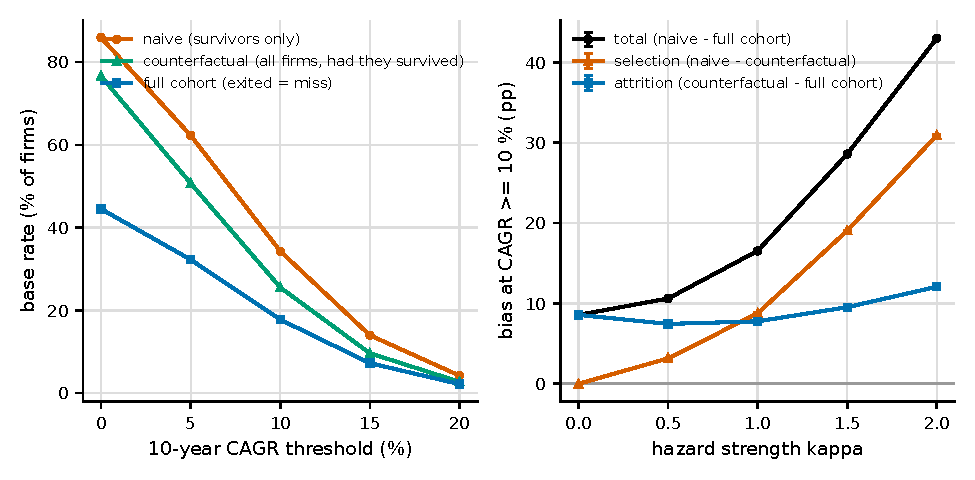
\includegraphics[width=\linewidth]{figures/fig7_survivorship.pdf}
\caption{Survivorship bias in 10-year growth base rates, synthetic universe of 2000 firms (M = 2000 cohorts, base hazard h0 = 0.04). Left: the naive, counterfactual and full-cohort base rates for kappa = 1. Right: at a CAGR threshold of 10\,\%, the total bias and its parts against the hazard strength: selection (survivors are not a random sample) and attrition (exited firms count as misses). Error bars $\pm 1.96$ se (Monte-Carlo noise only, mostly smaller than the markers); the size depends on the assumed hazard.}
\label{fig:fig7_survivorship}
\end{figure}

\begin{table}[H]
\centering
\scriptsize
\caption{Survivorship bias of 10-year growth base rates (in \%; synthetic universe of 2000 firms, M = 2000 cohorts per setting). Naive: survivors only (``what share of today's listed firms grew this fast?''). Counterfactual: all firms had they survived (``what share has the growth driver?''). Full cohort: exited firms count as misses (``how likely is a firm picked at the start to achieve it?''). Selection = naive $-$ counterfactual; attrition = counterfactual $-$ full cohort; total = their sum (percentage points $\pm$ Monte-Carlo se; the parameter choices dominate the size). Acquisitions are treated like failures.}
\label{tab:T6_survivorship}
\setlength{\tabcolsep}{3pt}
\begin{tabular}{rrrrrrrrrr}
\toprule
$h_0$ & $\kappa$ & Surv.\ (\%) & CAGR $\ge$ (\%) & Naive & Counterf. & Full cohort & Selection & Attrition & Total \\
\midrule
0 & 0 & 100.0 & 5 & 50.7 & 50.7 & 50.7 & 0.0 $\pm$ 0.00 & 0.0 $\pm$ 0.00 & 0.0 $\pm$ 0.00 \\
0 & 0 & 100.0 & 10 & 25.6 & 25.6 & 25.6 & 0.0 $\pm$ 0.00 & 0.0 $\pm$ 0.00 & 0.0 $\pm$ 0.00 \\
0 & 0 & 100.0 & 15 & 9.6 & 9.6 & 9.6 & 0.0 $\pm$ 0.00 & 0.0 $\pm$ 0.00 & 0.0 $\pm$ 0.00 \\
0.04 & 0 & 66.5 & 5 & 50.7 & 50.7 & 33.7 & -0.0 $\pm$ 0.02 & 17.0 $\pm$ 0.02 & 17.0 $\pm$ 0.02 \\
0.04 & 0 & 66.5 & 10 & 25.6 & 25.6 & 17.0 & -0.0 $\pm$ 0.02 & 8.6 $\pm$ 0.01 & 8.6 $\pm$ 0.01 \\
0.04 & 0 & 66.5 & 15 & 9.7 & 9.7 & 6.4 & -0.0 $\pm$ 0.01 & 3.2 $\pm$ 0.01 & 3.2 $\pm$ 0.01 \\
0.04 & 0.5 & 63.0 & 5 & 54.8 & 50.7 & 34.5 & 4.1 $\pm$ 0.02 & 16.2 $\pm$ 0.02 & 20.2 $\pm$ 0.02 \\
0.04 & 0.5 & 63.0 & 10 & 28.7 & 25.5 & 18.1 & 3.2 $\pm$ 0.02 & 7.4 $\pm$ 0.01 & 10.6 $\pm$ 0.01 \\
0.04 & 0.5 & 63.0 & 15 & 11.3 & 9.6 & 7.1 & 1.6 $\pm$ 0.01 & 2.5 $\pm$ 0.01 & 4.2 $\pm$ 0.01 \\
0.04 & 1 & 51.8 & 5 & 62.3 & 50.7 & 32.3 & 11.6 $\pm$ 0.02 & 18.4 $\pm$ 0.02 & 30.0 $\pm$ 0.02 \\
0.04 & 1 & 51.8 & 10 & 34.3 & 25.5 & 17.8 & 8.8 $\pm$ 0.02 & 7.8 $\pm$ 0.01 & 16.5 $\pm$ 0.02 \\
0.04 & 1 & 51.8 & 15 & 14.0 & 9.6 & 7.2 & 4.3 $\pm$ 0.01 & 2.4 $\pm$ 0.01 & 6.7 $\pm$ 0.01 \\
0.04 & 1.5 & 35.9 & 5 & 74.4 & 50.7 & 26.7 & 23.7 $\pm$ 0.03 & 24.0 $\pm$ 0.02 & 47.7 $\pm$ 0.03 \\
0.04 & 1.5 & 35.9 & 10 & 44.6 & 25.6 & 16.0 & 19.1 $\pm$ 0.03 & 9.5 $\pm$ 0.01 & 28.6 $\pm$ 0.03 \\
0.04 & 1.5 & 35.9 & 15 & 19.3 & 9.6 & 6.9 & 9.7 $\pm$ 0.02 & 2.7 $\pm$ 0.01 & 12.4 $\pm$ 0.02 \\
0.04 & 2 & 23.8 & 5 & 85.0 & 50.6 & 20.2 & 34.3 $\pm$ 0.04 & 30.4 $\pm$ 0.02 & 64.7 $\pm$ 0.03 \\
0.04 & 2 & 23.8 & 10 & 56.4 & 25.5 & 13.4 & 30.9 $\pm$ 0.04 & 12.1 $\pm$ 0.02 & 43.0 $\pm$ 0.04 \\
0.04 & 2 & 23.8 & 15 & 26.5 & 9.6 & 6.3 & 16.9 $\pm$ 0.04 & 3.3 $\pm$ 0.01 & 20.2 $\pm$ 0.03 \\
\bottomrule
\end{tabular}
\end{table}


% =====================================================================================
\section{Conceptual soundness}
\usertext{Assessment of the modelling choices: loss sign convention, quantile convention of historical
simulation, distributional assumptions, GARCH estimation (MLE, constraints, starts), the ES definition.}
\begin{figure}[H]
\centering
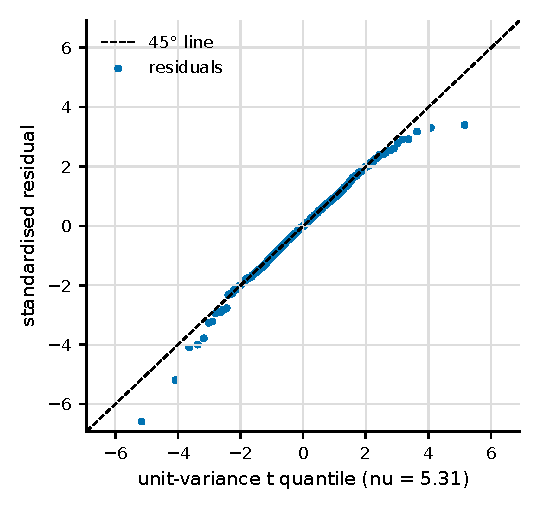
\includegraphics[width=0.55\linewidth]{figures/fig6_qq_residuals.pdf}
\caption{QQ plot of the standardised residuals of a GARCH(1,1)-t fit to one synthetic GARCH-t6 path (seed 20261110, n = 1000) against the fitted unit-variance t ($\hat\nu$ = 5.31); plotting positions $(i - 0.5)/n$.}
\label{fig:fig6_qq_residuals}
\end{figure}

\usertext{Interpretation of the QQ plot: are the fitted t tails adequate?}

% =====================================================================================
\section{Implementation verification}
\usertext{Testing approach: unit tests with independent checks (closed forms against numerical integration,
brute-force binomial sums, Monte-Carlo checks), look-ahead spy tests, reproducibility (fixed seeds; byte-identical
random streams within one numpy version, results files fingerprinted by the code that produced them), and the
independent code reviews; the number of tests and where they run.}

% =====================================================================================
\section{Outcome analysis and backtesting}
\begin{figure}[H]
\centering
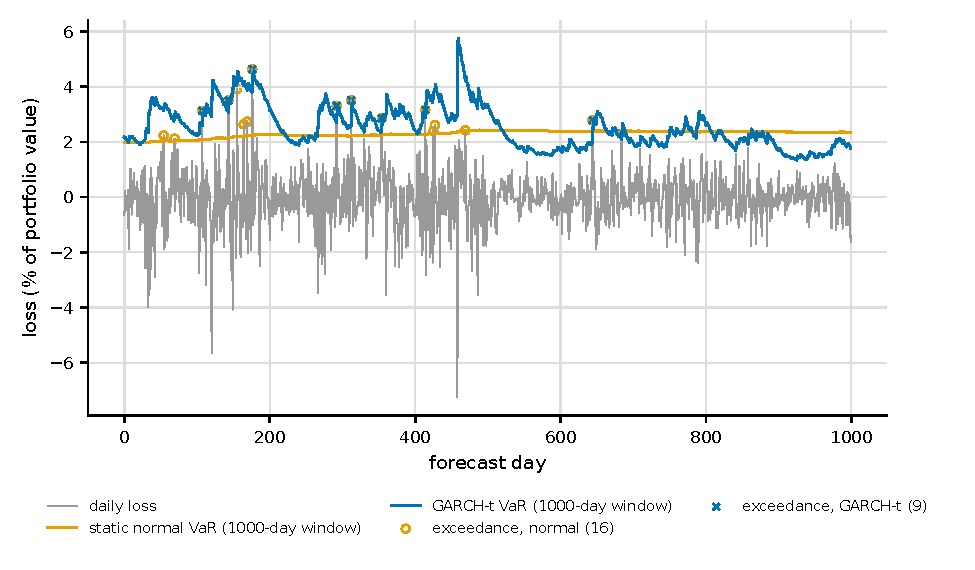
\includegraphics[width=\linewidth]{figures/fig1_exceedances.pdf}
\caption{One synthetic GARCH(1,1)-t6 path (seed 20261109, 1000 forecast days): daily losses, the 99\,\% VaR of a static normal model (1000-day window) and of GARCH(1,1)-t (1000-day window), and their exceedances (normal 16, GARCH-t 9; expected 10). Both models use the same estimation window, so only the model differs. One path only: the counts illustrate clustering, they are not a test.}
\label{fig:fig1_exceedances}
\end{figure}

\usertext{Reading of the exceedance plot: clustering of the static-normal exceedances against the GARCH-t
forecast.}
\begin{table}[H]
\centering
\small
\caption{Size of the backtests at 5\,\% (rejection rate of a correct VaR / ES, in \%). Exact binomial sums; oracle rows: M = 1000 synthetic replications ($\pm$ se).}
\label{tab:T2_size}
\begin{tabular}{lrrrr}
\toprule
 & Kupiec & Binomial exact & Christoffersen cc & ES Z2 \\
\midrule
exact size, T = 250 & 9.48 & 4.12 & -- & -- \\
exact size, T = 1000 & 5.51 & 3.65 & -- & -- \\
\midrule
oracle, garch\_normal, T = 250 & 10.6 $\pm$ 1.0 & 4.5 $\pm$ 0.7 & 1.0 $\pm$ 0.3 & 4.6 $\pm$ 0.7 \\
oracle, garch\_normal, T = 1000 & 6.2 $\pm$ 0.8 & 4.6 $\pm$ 0.7 & 2.8 $\pm$ 0.5 & 4.6 $\pm$ 0.7 \\
oracle, garch\_t6, T = 250 & 9.6 $\pm$ 0.9 & 3.8 $\pm$ 0.6 & 1.0 $\pm$ 0.3 & 4.4 $\pm$ 0.6 \\
oracle, garch\_t6, T = 1000 & 4.6 $\pm$ 0.7 & 2.5 $\pm$ 0.5 & 1.7 $\pm$ 0.4 & 4.6 $\pm$ 0.7 \\
oracle, iid\_normal, T = 250 & 8.7 $\pm$ 0.9 & 5.3 $\pm$ 0.7 & 1.1 $\pm$ 0.3 & 6.4 $\pm$ 0.8 \\
oracle, iid\_normal, T = 1000 & 5.7 $\pm$ 0.7 & 4.1 $\pm$ 0.6 & 2.7 $\pm$ 0.5 & 4.8 $\pm$ 0.7 \\
oracle, iid\_t5, T = 250 & 9.0 $\pm$ 0.9 & 4.0 $\pm$ 0.6 & 1.0 $\pm$ 0.3 & 5.1 $\pm$ 0.7 \\
oracle, iid\_t5, T = 1000 & 7.4 $\pm$ 0.8 & 5.0 $\pm$ 0.7 & 4.1 $\pm$ 0.6 & 6.5 $\pm$ 0.8 \\
oracle, regime, T = 250 & 10.5 $\pm$ 1.0 & 4.3 $\pm$ 0.6 & 1.0 $\pm$ 0.3 & 5.0 $\pm$ 0.7 \\
oracle, regime, T = 1000 & 5.1 $\pm$ 0.7 & 3.4 $\pm$ 0.6 & 2.6 $\pm$ 0.5 & 4.4 $\pm$ 0.6 \\
\bottomrule
\end{tabular}
\end{table}

\usertext{Size of the tests: why Kupiec over-rejects at T = 250 and what that means for a one-year backtest.}
\begin{figure}[H]
\centering
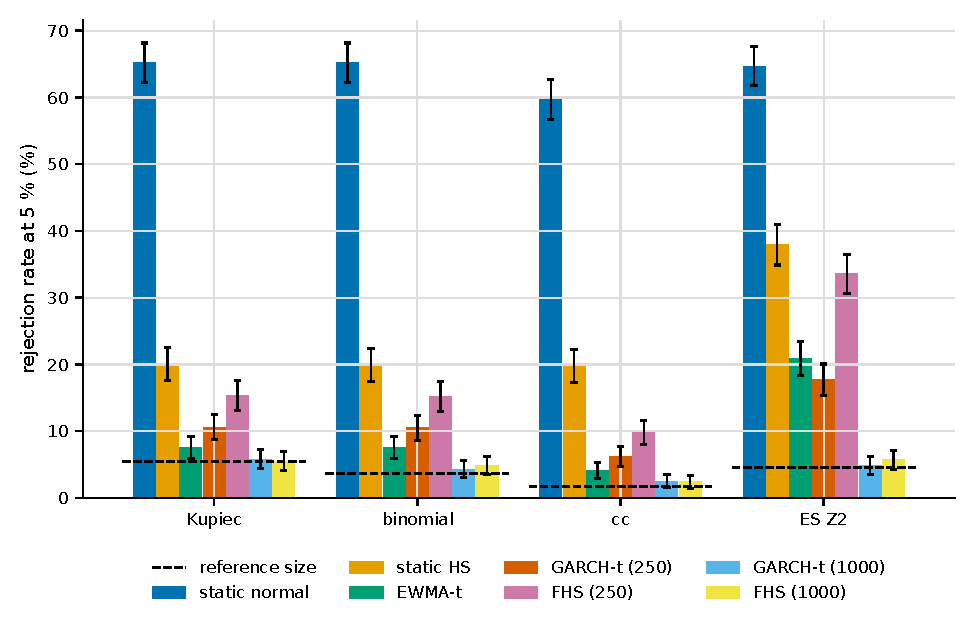
\includegraphics[width=\linewidth]{figures/fig2_rejection_rates.pdf}
\caption{Rejection rates of the VaR tests (Kupiec, exact binomial, Christoffersen cc; 99\,\%) and the Acerbi--Sz\'ekely Z2 ES test (97.5\,\%) on synthetic GARCH(1,1)-t6 data, T = 1000, M = 1000 replications; error bars $\pm 1.96$ se. Dashed lines: the reference size of each test (exact size for Kupiec and binomial, oracle rate for cc and Z2). Numbers in brackets: estimation window in days.}
\label{fig:fig2_rejection_rates}
\end{figure}

\begin{table}[H]
\centering
\scriptsize
\caption{Rejection rates (\%, $\pm$ se) of the backtests at 5\,\% by data, model and estimation window; M = 1000 synthetic replications. Not size-adjusted: compare with Table~\ref{tab:T2_size}.}
\label{tab:T3_power}
\begin{tabular}{llrrrrrrr}
\toprule
Data & Model & Window & T & Exceed.\ (\%) & Kupiec & Binomial & cc & Z2 \\
\midrule
iid\_t5 & normal & 250 & 250 & 1.58 & 10.8 $\pm$ 1.0 & 19.2 $\pm$ 1.2 & 5.4 $\pm$ 0.7 & 18.2 $\pm$ 1.2 \\
garch\_t6 & normal & 250 & 250 & 1.85 & 27.5 $\pm$ 1.4 & 32.4 $\pm$ 1.5 & 20.8 $\pm$ 1.3 & 32.2 $\pm$ 1.5 \\
garch\_t6 & hs & 250 & 250 & 1.35 & 19.3 $\pm$ 1.2 & 17.4 $\pm$ 1.2 & 9.8 $\pm$ 0.9 & 24.5 $\pm$ 1.4 \\
garch\_t6 & ewma\_t & 250 & 250 & 1.28 & 6.3 $\pm$ 0.8 & 9.1 $\pm$ 0.9 & 1.9 $\pm$ 0.4 & 11.1 $\pm$ 1.0 \\
garch\_t6 & garch\_t & 250 & 250 & 1.25 & 12.0 $\pm$ 1.0 & 11.7 $\pm$ 1.0 & 4.0 $\pm$ 0.6 & 12.2 $\pm$ 1.0 \\
garch\_t6 & fhs & 250 & 250 & 1.35 & 11.1 $\pm$ 1.0 & 14.1 $\pm$ 1.1 & 4.9 $\pm$ 0.7 & 16.9 $\pm$ 1.2 \\
regime & normal & 250 & 250 & 2.27 & 37.8 $\pm$ 1.5 & 48.2 $\pm$ 1.6 & 37.1 $\pm$ 1.5 & 43.5 $\pm$ 1.6 \\
regime & hs & 250 & 250 & 1.35 & 14.6 $\pm$ 1.1 & 16.5 $\pm$ 1.2 & 10.3 $\pm$ 1.0 & 25.0 $\pm$ 1.4 \\
regime & ewma\_t & 250 & 250 & 1.33 & 6.3 $\pm$ 0.8 & 10.5 $\pm$ 1.0 & 4.3 $\pm$ 0.6 & 13.9 $\pm$ 1.1 \\
regime & garch\_t & 250 & 250 & 1.24 & 11.6 $\pm$ 1.0 & 11.1 $\pm$ 1.0 & 4.9 $\pm$ 0.7 & 12.2 $\pm$ 1.0 \\
regime & fhs & 250 & 250 & 1.36 & 10.9 $\pm$ 1.0 & 14.2 $\pm$ 1.1 & 5.7 $\pm$ 0.7 & 17.5 $\pm$ 1.2 \\
\midrule
iid\_t5 & normal & 250 & 1000 & 1.58 & 40.6 $\pm$ 1.6 & 40.6 $\pm$ 1.6 & 24.5 $\pm$ 1.4 & 35.6 $\pm$ 1.5 \\
garch\_t6 & normal & 250 & 1000 & 1.87 & 65.2 $\pm$ 1.5 & 65.2 $\pm$ 1.5 & 59.7 $\pm$ 1.6 & 64.7 $\pm$ 1.5 \\
garch\_t6 & hs & 250 & 1000 & 1.38 & 20.1 $\pm$ 1.3 & 19.9 $\pm$ 1.3 & 19.8 $\pm$ 1.3 & 37.9 $\pm$ 1.5 \\
garch\_t6 & ewma\_t & 250 & 1000 & 1.24 & 7.6 $\pm$ 0.8 & 7.5 $\pm$ 0.8 & 4.1 $\pm$ 0.6 & 20.9 $\pm$ 1.3 \\
garch\_t6 & garch\_t & 250 & 1000 & 1.25 & 10.6 $\pm$ 1.0 & 10.5 $\pm$ 1.0 & 6.2 $\pm$ 0.8 & 17.7 $\pm$ 1.2 \\
garch\_t6 & fhs & 250 & 1000 & 1.35 & 15.3 $\pm$ 1.1 & 15.2 $\pm$ 1.1 & 9.8 $\pm$ 0.9 & 33.6 $\pm$ 1.5 \\
garch\_t6 & garch\_t & 1000 & 1000 & 1.03 & 5.8 $\pm$ 0.7 & 4.3 $\pm$ 0.6 & 2.5 $\pm$ 0.5 & 4.9 $\pm$ 0.7 \\
garch\_t6 & fhs & 1000 & 1000 & 1.12 & 5.5 $\pm$ 0.7 & 4.9 $\pm$ 0.7 & 2.4 $\pm$ 0.5 & 5.7 $\pm$ 0.7 \\
regime & normal & 250 & 1000 & 2.28 & 92.4 $\pm$ 0.8 & 92.4 $\pm$ 0.8 & 89.6 $\pm$ 1.0 & 86.8 $\pm$ 1.1 \\
regime & hs & 250 & 1000 & 1.35 & 16.1 $\pm$ 1.2 & 16.1 $\pm$ 1.2 & 21.6 $\pm$ 1.3 & 38.8 $\pm$ 1.5 \\
regime & ewma\_t & 250 & 1000 & 1.37 & 19.4 $\pm$ 1.3 & 19.1 $\pm$ 1.2 & 19.2 $\pm$ 1.2 & 35.1 $\pm$ 1.5 \\
regime & garch\_t & 250 & 1000 & 1.27 & 12.8 $\pm$ 1.1 & 12.4 $\pm$ 1.0 & 9.5 $\pm$ 0.9 & 18.0 $\pm$ 1.2 \\
regime & fhs & 250 & 1000 & 1.37 & 17.4 $\pm$ 1.2 & 17.4 $\pm$ 1.2 & 12.2 $\pm$ 1.0 & 34.7 $\pm$ 1.5 \\
\bottomrule
\end{tabular}
\end{table}

\begin{figure}[H]
\centering
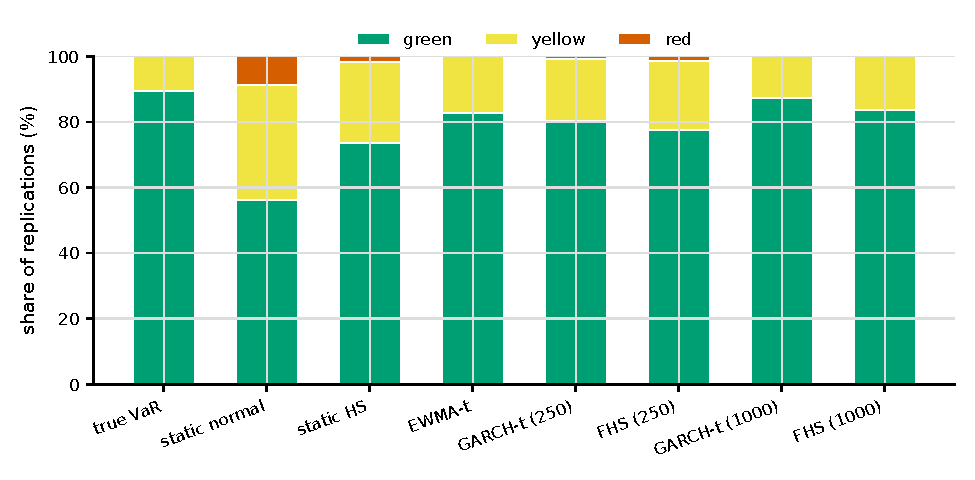
\includegraphics[width=\linewidth]{figures/fig4_traffic_light.pdf}
\caption{Basel traffic-light zones (last 250 forecast days, 99\,\% VaR) per model on synthetic GARCH(1,1)-t6 data, T = 1000, M = 1000. Numbers in brackets: estimation window in days.}
\label{fig:fig4_traffic_light}
\end{figure}

\usertext{Power and the comparison of static and conditional models; the ES test against the VaR tests;
the traffic light as the regulatory view.}

% =====================================================================================
\section{Benchmarking and sensitivity}
\subsection{Estimation window}
\begin{figure}[H]
\centering
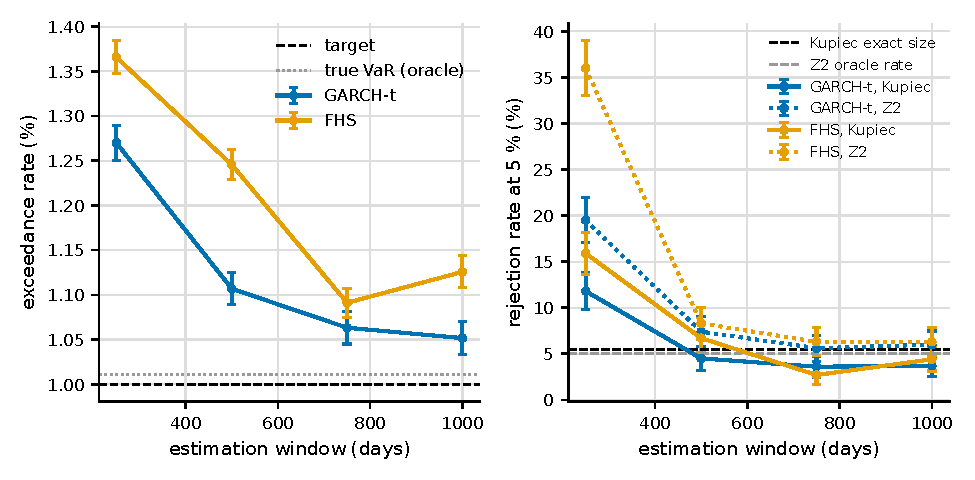
\includegraphics[width=\linewidth]{figures/fig3_estimation_window.pdf}
\caption{Estimation risk against the window length: correctly specified GARCH(1,1)-t and FHS on synthetic GARCH-t6 data, T = 1000 (the same forecast days for every window), M = 1000. Left: exceedance rate of the 99\,\% VaR, with the target and the oracle rate (the left axis does not start at 0); right: Kupiec and Z2 rejection rates with their reference sizes. Error bars $\pm 1.96$ se.}
\label{fig:fig3_estimation_window}
\end{figure}

\begin{table}[H]
\centering
\scriptsize
\caption{Estimation window: correctly specified GARCH(1,1)-t and FHS on synthetic GARCH-t6 data, T = 1000 (same forecast days for every window), M = 1000; rates in \% ($\pm$ se). Reference sizes: Kupiec 5.51, binomial 3.65 (exact); cc and Z2: the true-VaR row. $\Delta$: paired difference of the exceedance rate against the true VaR on the same days (percentage points $\pm$ se); positive = anti-conservative. The 1000-day rows use the same design as the 1000-day rows of the power study (checked per replication); only the data seeds differ, so differences between the two studies are Monte-Carlo noise.}
\label{tab:T4_estimation_window}
\setlength{\tabcolsep}{3.5pt}
\begin{tabular}{lrrrrrrrr}
\toprule
Model & Window & Exceed.\ (\%) & $\Delta$ exceed.\ (pp) & Kupiec & Binomial & cc & Z2 & VaR error (\%) \\
\midrule
true VaR & -- & 1.01 $\pm$ 0.01 & -- & 4.7 $\pm$ 0.7 & 3.4 $\pm$ 0.6 & 2.0 $\pm$ 0.4 & 5.0 $\pm$ 0.7 & 0.0 \\
garch\_t & 250 & 1.27 $\pm$ 0.01 & +0.259 $\pm$ 0.010 & 11.8 $\pm$ 1.0 & 11.6 $\pm$ 1.0 & 6.7 $\pm$ 0.8 & 19.5 $\pm$ 1.3 & 11.6 \\
garch\_t & 500 & 1.11 $\pm$ 0.01 & +0.096 $\pm$ 0.008 & 4.5 $\pm$ 0.7 & 4.2 $\pm$ 0.6 & 2.4 $\pm$ 0.5 & 7.4 $\pm$ 0.8 & 7.5 \\
garch\_t & 750 & 1.06 $\pm$ 0.01 & +0.052 $\pm$ 0.007 & 3.6 $\pm$ 0.6 & 2.7 $\pm$ 0.5 & 2.2 $\pm$ 0.5 & 5.6 $\pm$ 0.7 & 6.0 \\
garch\_t & 1000 & 1.05 $\pm$ 0.01 & +0.041 $\pm$ 0.007 & 3.7 $\pm$ 0.6 & 2.9 $\pm$ 0.5 & 2.4 $\pm$ 0.5 & 6.0 $\pm$ 0.8 & 5.1 \\
fhs & 250 & 1.37 $\pm$ 0.01 & +0.355 $\pm$ 0.013 & 15.9 $\pm$ 1.2 & 15.9 $\pm$ 1.2 & 9.8 $\pm$ 0.9 & 36.0 $\pm$ 1.5 & 15.5 \\
fhs & 500 & 1.25 $\pm$ 0.01 & +0.235 $\pm$ 0.011 & 6.7 $\pm$ 0.8 & 6.7 $\pm$ 0.8 & 5.1 $\pm$ 0.7 & 8.3 $\pm$ 0.9 & 10.5 \\
fhs & 750 & 1.09 $\pm$ 0.01 & +0.080 $\pm$ 0.010 & 2.7 $\pm$ 0.5 & 2.4 $\pm$ 0.5 & 1.6 $\pm$ 0.4 & 6.3 $\pm$ 0.8 & 8.7 \\
fhs & 1000 & 1.13 $\pm$ 0.01 & +0.115 $\pm$ 0.010 & 4.4 $\pm$ 0.6 & 4.3 $\pm$ 0.6 & 2.9 $\pm$ 0.5 & 6.3 $\pm$ 0.8 & 7.3 \\
\bottomrule
\end{tabular}
\end{table}

\usertext{How the over-rejection of the correct model falls with the window length, why the VaR stays slightly
anti-conservative even where the rejection rates are back at the reference size (paired exceedance difference),
and the recommended window.}
\subsection{10-day horizon}
\begin{figure}[H]
\centering
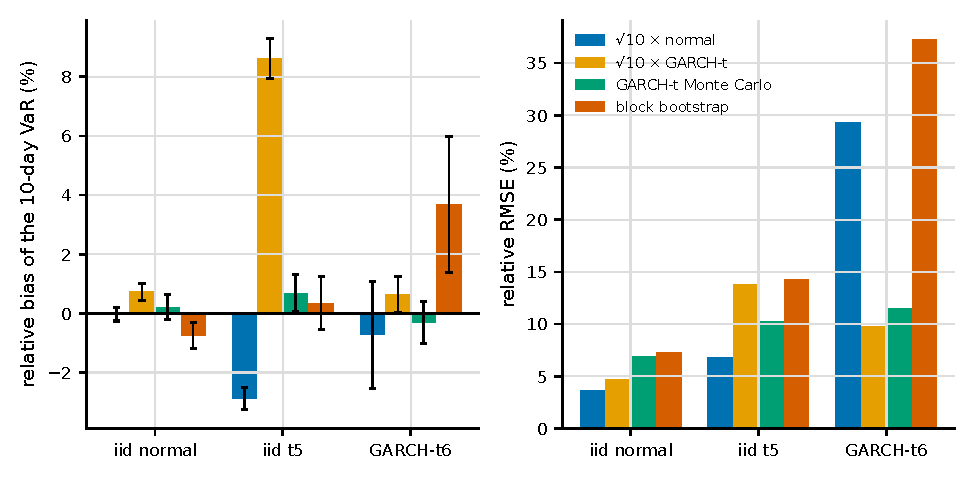
\includegraphics[width=\linewidth]{figures/fig5_horizon.pdf}
\caption{10-day 99\,\% VaR against the true 10-day VaR: relative bias ($\pm 1.96$ se) and relative RMSE per method and synthetic data set; 500-day window, M = 1000.}
\label{fig:fig5_horizon}
\end{figure}

\begin{table}[H]
\centering
\small
\caption{10-day 99\,\% VaR against the true 10-day VaR (relative, in \%; $\pm$ se over M = 1000 replications). MC se: simulation error of the estimate and of the truth.}
\label{tab:T5_horizon}
\begin{tabular}{llrrrr}
\toprule
Data & Method & Bias & RMSE & Est.\ MC se & Truth MC se \\
\midrule
iid\_normal & sqrt10\_normal & -0.0 $\pm$ 0.1 & 3.6 & -- & 0.00 \\
iid\_normal & sqrt10\_garch & +0.7 $\pm$ 0.1 & 4.7 & -- & 0.00 \\
iid\_normal & garch\_mc & +0.2 $\pm$ 0.2 & 6.9 & 1.18 & 0.00 \\
iid\_normal & bootstrap & -0.8 $\pm$ 0.2 & 7.3 & 1.15 & 0.00 \\
iid\_t5 & sqrt10\_normal & -2.9 $\pm$ 0.2 & 6.8 & -- & 0.84 \\
iid\_t5 & sqrt10\_garch & +8.6 $\pm$ 0.3 & 13.8 & -- & 0.84 \\
iid\_t5 & garch\_mc & +0.7 $\pm$ 0.3 & 10.2 & 1.41 & 0.84 \\
iid\_t5 & bootstrap & +0.3 $\pm$ 0.5 & 14.3 & 1.31 & 0.84 \\
garch\_t6 & sqrt10\_normal & -0.7 $\pm$ 0.9 & 29.3 & -- & 1.01 \\
garch\_t6 & sqrt10\_garch & +0.6 $\pm$ 0.3 & 9.8 & -- & 1.01 \\
garch\_t6 & garch\_mc & -0.3 $\pm$ 0.4 & 11.5 & 1.60 & 1.01 \\
garch\_t6 & bootstrap & +3.7 $\pm$ 1.2 & 37.2 & 1.44 & 1.01 \\
\bottomrule
\end{tabular}
\end{table}

\usertext{Square-root-of-time against simulation and bootstrap: when the approximation is acceptable.}

% =====================================================================================
\section{Limitations}
\usertext{Synthetic data only; univariate; fixed parameters of the data-generating processes; Monte-Carlo
error of the study results (see the $\pm$ se); what a validation on real data would add.}

% =====================================================================================
\section{Findings and recommendations}
\usertext{How the severities were set (definitions of High / Medium / Low) and the overall rating.}
\begin{table}[H]
\centering
\scriptsize
\caption{Findings register. Severities are PROPOSED and must be confirmed by the validator.}
\label{tab:T7_findings}
\begin{tabular}{>{\raggedright\arraybackslash}p{0.5cm}>{\raggedright\arraybackslash}p{5.2cm}>{\raggedright\arraybackslash}p{1.8cm}>{\raggedright\arraybackslash}p{2.7cm}>{\raggedright\arraybackslash}p{3.5cm}}
\toprule
ID & Finding & Severity & Evidence & Proposed remediation \\
\midrule
F1 & With a 250-day window the correctly specified GARCH(1,1)-t over-rejects: Kupiec 10.6 $\pm$ 1.0\,\% vs exact size 5.5\,\%, Z2 17.7 $\pm$ 1.2\,\% (T = 1000); exceedance rate 1.25\,\%. With 1000 days: Kupiec 5.8 $\pm$ 0.7\,\%. Estimation-window study: the rejection rates fall to about the reference size by 500 days (GARCH-t) and 750 days (FHS) (Kupiec, \% by window: 250: 11.8, 500: 4.5, 750: 3.6, 1000: 3.7), but the VaR stays slightly anti-conservative: exceedance rate 1.05--1.13\,\% against the true VaR's 1.01\,\% (GARCH-t by window: 250: 1.27, 500: 1.11, 750: 1.06, 1000: 1.05). Paired difference against the true VaR at 1000 days: +0.041 $\pm$ 0.007 pp. & PROPOSED: High & Tab.~\ref{tab:T3_power}, \ref{tab:T4_estimation_window}; Fig.~\ref{fig:fig3_estimation_window} & Estimation window of at least 500 days for GARCH-t and 750 days for FHS (where the rejection rates reach the reference sizes); account for the remaining small anti-conservatism (parameter uncertainty), e.g. by a VaR add-on or a longer window. \\
F2 & FHS with a 250-day window underestimates the tail (ES): Z2 rejects in 33.6 $\pm$ 1.5\,\% (oracle 4.6\,\%, T = 1000); with 750 days 6.3 $\pm$ 0.8\,\%. & PROPOSED: Medium & Tab.~\ref{tab:T3_power}, \ref{tab:T4_estimation_window} & Longer window for the residual distribution; monitor the ES backtest separately from VaR. \\
F3 & Static models miss volatility clustering: the static normal VaR on GARCH-t data is rejected by cc in 59.7 $\pm$ 1.6\,\% and by Z2 in 64.7 $\pm$ 1.5\,\% (T = 1000). & PROPOSED: High & Fig.~\ref{fig:fig1_exceedances}, \ref{fig:fig2_rejection_rates}; Tab.~\ref{tab:T3_power} & Use a conditional volatility model (GARCH-t / FHS with an adequate window). \\
F4 & The Kupiec test is mis-sized at T = 250: exact size 9.48\,\% at a nominal 5\,\% (x = 0 is rejected); the exact binomial test keeps 4.12\,\%. & PROPOSED: Medium & Tab.~\ref{tab:T2_size} & Report the exact binomial test (or the exact size) alongside Kupiec for one-year backtests. \\
F5 & The Christoffersen independence test is undersized (0.9--2.6\,\% on correct VaRs) and has little power on its own. & PROPOSED: Low & Results file of the power study (ind columns) & Do not rely on the independence test alone; use cc and the ES test. \\
F6 & $\sqrt{10}$ scaling of a fat-tailed one-day VaR overstates the 10-day VaR on iid t5 data (+8.6 $\pm$ 0.3\,\%). On GARCH-t6 data $\sqrt{10}$ is unbiased on average but $\sqrt{10}\times$ static normal has an RMSE of 29.3\,\%. & PROPOSED: Medium & Fig.~\ref{fig:fig5_horizon}; Tab.~\ref{tab:T5_horizon} & Simulate the 10-day distribution (GARCH Monte Carlo); use $\sqrt{10}$ only for a conditional one-day VaR when the 10-day sum is near-normal. \\
F7 & The stationary block bootstrap is biased on GARCH-t6 data (+3.7 $\pm$ 1.2\,\%, RMSE 37.2\,\%): it does not condition on the current volatility. & PROPOSED: Low & Tab.~\ref{tab:T5_horizon} & Do not use the unconditional bootstrap as the 10-day benchmark under volatility clustering. \\
F8 & Historical simulation with $k = \lceil n\alpha\rceil$ has a finite-sample exceedance probability of $(n-k+1)/(n+1)$ = 1.20\,\% at n = 250, $\alpha$ = 0.99 (simulated: 1.21\,\% on iid normal data). & PROPOSED: Low & Results of the power study (HS on iid normal data) & Document the quantile convention; consider a longer window or interpolation. \\
F9 & Survivorship (synthetic, hazard strength 1, CAGR $\ge$ 10\,\%): a survivors-only database shows 34.3\,\%, against 25.5\,\% for all firms had they survived (selection bias 8.8 $\pm$ 0.02 pp) and 17.8\,\% for the full cohort with exits as misses (attrition 7.8 $\pm$ 0.01 pp). The size depends on the assumed hazard; the $\pm$ se is Monte-Carlo noise only. & PROPOSED: Medium & Fig.~\ref{fig:fig7_survivorship}; Tab.~\ref{tab:T6_survivorship} & Use point-in-time data that include delisted firms, and state which base rate (counterfactual or full cohort) answers the question asked. \\
\bottomrule
\end{tabular}
\end{table}

\usertext{Recommendations and follow-ups, with owners and dates.}

% =====================================================================================
\appendix
\section{Formulas and test definitions}
Losses are positive: $L = -r$. For a confidence level $\alpha$,
$\mathrm{VaR}_\alpha = F_L^{-1}(\alpha)$ and $\mathrm{ES}_\alpha = \mathrm{E}[L \mid L \ge \mathrm{VaR}_\alpha]$.

\paragraph{Kupiec (proportion of failures).} With $T$ days, $x$ exceedances, $p = 1-\alpha$, $\hat p = x/T$:
\[ LR_{uc} = -2\ln\frac{(1-p)^{T-x}p^{x}}{(1-\hat p)^{T-x}\hat p^{x}} \sim \chi^2_1 . \]

\paragraph{Exact binomial test.} Two-sided p-value: the total probability under $\mathrm{Bin}(T, p)$ of all
counts at most as likely as $x$.

\paragraph{Christoffersen.} With transition counts $n_{ij}$,
$LR_{ind} = -2\ln[L(\hat\pi)/L(\hat\pi_{01},\hat\pi_{11})] \sim \chi^2_1$ and
$LR_{cc} = LR_{uc} + LR_{ind} \sim \chi^2_2$, both on the $T-1$ transitions.

\paragraph{Acerbi--Sz\'ekely Z2 (loss sign).}
\[ Z_2 = \sum_{t=1}^{T} \frac{L_t I_t}{T(1-\alpha)\,\mathrm{ES}_t} - 1, \qquad I_t = \mathbf{1}\{L_t > \mathrm{VaR}_t\}; \]
$Z_2 > 0$ indicates underestimated ES; the p-value is simulated under each day's predictive distribution.

\paragraph{GARCH(1,1).} $L_t = \mu + \sigma_t z_t$,
$\sigma_t^2 = \omega + \alpha (L_{t-1}-\mu)^2 + \beta\sigma_{t-1}^2$, $z_t$ unit-variance $t_\nu$.

\paragraph{Basel traffic light.} Zones from the binomial CDF of the exceedances in 250 days:
green below 95\,\%, red from 99.99\,\%.

\usertext{Any further derivations the author wants to include (e.g. the normal and t ES formulas).}

\section{Reproduction}
From \texttt{UFOS.ai/RiskLab/}:
\begin{verbatim}
python -m unittest discover -s tests
python studies/var_backtest_power.py --mode full --save-results
python studies/horizon_10d.py --mode full --save-results
python studies/estimation_window.py --mode full --save-results
python studies/survivorship.py --mode full --save-results
python report/build_report.py   # -> out/report/validation_report.pdf
\end{verbatim}
{\sloppy Each study command also takes the option \texttt{--save-results}, which writes its full-run
results to the folder \texttt{studies/results/}. The study results used here are stored there, each with a
fingerprint of the code that produced it; the build refuses results whose fingerprint does not match the
current code.\par}

\end{document}
